\documentclass[default]{beamer}
\setbeamertemplate{navigation symbols}{}

\usetheme{Frankfurt}
%\useoutertheme{infolines}
\usecolortheme{beaver}

\usepackage[utf8]{inputenc}					% Выбор языка и кодировки
\usepackage[english]{babel}	% Языки: русский, английский
\usepackage{csquotes}
\usepackage{tikz}
\usetikzlibrary{arrows,shapes,calc}
\usepackage{animate}
\usepackage{fp}
\usepackage{textpos}

\usepackage[
	language=auto,
	autolang=other,
	backend=biber,
	style=authortitle,
	sorting=ydnt,
	maxbibnames=5
]{biblatex}
\addbibresource{strl_cai16.bib}
				
\DeclareSourcemap{
	\maps[datatype=bibtex, overwrite]{
		\map{
			\step[fieldset=langid, fieldvalue=english]
			\step[fieldset=doi, null]
			\step[fieldset=issn, null]
			\step[fieldset=isbn, null]
			\step[fieldset=url, null]
			\step[fieldsource=language, fieldset=langid, origfieldval]
		}
	}
}
\DeclareBibliographyDriver{std}{%
	\usebibmacro{bibindex}%
	\usebibmacro{begentry}%
	\usebibmacro{author/editor+others/translator+others}%
	\setunit{\labelnamepunct}\newblock
	\usebibmacro{title}%
	\newunit\newblock
	\usebibmacro{maintitle+booktitle}
	\newunit\newblock
	\usebibmacro{journal}%
	\newunit\newblock
	\usebibmacro{date}%
	\newunit\newblock
	\usebibmacro{finentry}
}
\DeclareBibliographyAlias{article}{std}
\DeclareBibliographyAlias{book}{std}
\DeclareBibliographyAlias{inproceedings}{std}
\DeclareBibliographyAlias{incollection}{std}

\graphicspath{{../../images/}} 			% Пути к изображениям

\makeatletter
\setbeamertemplate{footline}
{
	\leavevmode%
	\hbox{%
		\begin{beamercolorbox}[wd=.333333\paperwidth,ht=2.25ex,dp=1ex,center]{author
				in head/foot}%
			\usebeamerfont{author in
				head/foot}\insertshortauthor~~\beamer@ifempty{\insertshortinstitute}{}{(\insertshortinstitute)}
		\end{beamercolorbox}%
		\begin{beamercolorbox}[wd=.333333\paperwidth,ht=2.25ex,dp=1ex,center]{title in
				head/foot}%
			\usebeamerfont{title in head/foot}\insertshorttitle
		\end{beamercolorbox}%
		\begin{beamercolorbox}[wd=.333333\paperwidth,ht=2.25ex,dp=1ex,right]{date in
				head/foot}%
			\usebeamerfont{date in head/foot}\insertshortdate{}\hspace*{2em}
			\insertframenumber{}\hspace*{2ex} 
		\end{beamercolorbox}
	}%
	\vskip0pt%
}

\renewcommand*{\bibfont}{\tiny}
\setlength\bibitemsep{-5pt}

\begin{document}
	
	\title[Introduction to AI]{Introduction to Artificial Intelligence: Methods, Models, Algorithms}
	\author[Panov]{\textbf{Aleksandr I. Panov and Konstantin S. Yakovlev}}
	\institute[HSE]{National Research University Higher School of Economics}
	\date{18 July 2018 -- Summer University} 
	
	{
	\setbeamertemplate{headline}{}
	\begin{frame}
		
		\titlepage
		\centering
		\href{mailto:apanov@hse.ru}{apanov@hse.ru}
		
		
\includegraphics[width=25pt]{misc/logos/hse.png} \hspace{10pt}
		\includegraphics[width=100pt]{misc/logos/ras.png} \hspace{10pt}
		
\includegraphics[width=80pt]{misc/logos/frccsc.png}
		
	\end{frame}
	}	

	\begin{frame}
		\frametitle{Self-presentation}
		\scriptsize
		\begin{columns}
			\begin{column}{0.85\textwidth}
				\textbf{Aleksandr I. Panov, PhD}
				\begin{itemize}
					\item Graduate of MIPT and NSU.
					\item Senior researcher of the Department ``Intelligent dynamic systems and cognitive research`` of FRC CSC RAS.
					\item Researcher and associate professor of HSE.
					\item Associate professor of Systems research at the Moscow Institute of physics and technology (MIPT).
					\item Member of the Russian Association of Artificial Intelligence (RAAI).
					\item Member of the Biologically inspired cognitive architectures Society (BICA Society).
					\item Participation in the organization of international schools and conferences on Biologically inspired cognitive architectures (BICA-2016 --- New York, BICA-2017 --- Moscow, Fierces on BICA), school of young scientists on AI (ISyT-2017, St. Petersburg), national AI conference (RCAI-2018).
					\item Member of the editorial Board of the journal Biologically Inspired Cognitive Architectures.
					\item Recipient of the medal of RAS for young scientists 2017.
					\item Mentor of the student laboratory for AI (SLabAI).
				\end{itemize}
			\end{column}
			
			\begin{column}{0.15\textwidth}
				\centering
				\includegraphics[width=\textwidth]{misc/logos/ras.png}
				\vspace{7pt}
				
\includegraphics[width=\textwidth]{misc/logos/frccsc.png}
				\vspace{7pt}
				\includegraphics[width=0.7\textwidth]{misc/logos/isa.png}
				\vspace{7pt}
				\includegraphics[width=0.5\textwidth]{misc/logos/raai.png}
				\vspace{7pt}
				
\includegraphics[width=0.5\textwidth]{misc/logos/hse.png}
				\vspace{7pt}
				\includegraphics[width=\textwidth]{misc/logos/mipt.jpg}
				\vspace{5pt}
				\includegraphics[width=\textwidth]{misc/logos/BICA.png}
				\vspace{5pt}
				\includegraphics[width=0.7\textwidth]{misc/logos/slabai3.png}
			\end{column}
			
		\end{columns}
	\end{frame}

	\begin{frame}
		\frametitle{Defenitions of AI}
		
		\begin{itemize}
			\onslide<1->{
				\item AI - is a scientific direction in which the tasks of hardware or software modeling of those types of human activity that are traditionally considered as intelligent are set and solved (Explanatory dictionary on AI).
			}
			\onslide<2->{
				\item  AI - is the science and technology of creating intelligent machines, especially intelligent computer programs (John McCarthy).
			}
			\onslide<3->{
				\item AI - is the science of ``intelligent agents'', i.e. a device or program that perceives its environment and takes actions that maximize its chances of success in achieving some goal (Russell and Norvig).
			}
		\end{itemize}
		\end{frame}
		
		
		\begin{frame}
		\frametitle{Cognitive sciences}
		
		
		\centering
		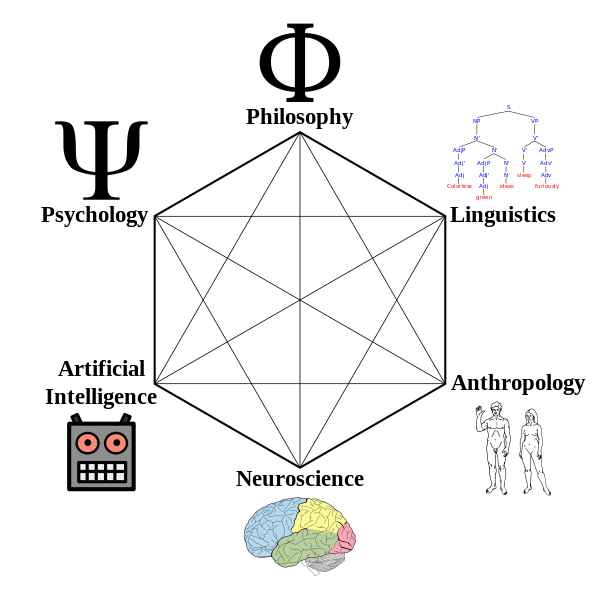
\includegraphics[width=0.5\textwidth]{cogsci.png}
		
		Cognitive science (lat. cognitio ``knowledge'') - interdisciplinary scientific direction studying the psyche, the mind of man and processes implemented it.
	\end{frame}

	\section{Little history}
	\subsection{1.1}
	\begin{frame}
		\frametitle{How did it happen}

		\begin{itemize}
			\item \textbf{1954} --- \textit{Rand Corporation}, \textit{Allen Newell}, \textit{John Shaw} and \textit{Herbert Simon}  --- chess program. \textit{Alan Turing}, \textit{Claude Shannon} and a group of Dutch psychologists volunteered to help.
			\item \textbf{1957} --- the chess program (NSS) was written. It used heuristics.
		\end{itemize}
	\end{frame}
	\subsection{1.2}
	\begin{frame}
	\frametitle{What happened next}
	
		\begin{itemize}
			\item \textbf{1960}  --- GPS (``general problem solver''): calculation of indefinite integrals, puzzles and some other tasks.  Programs of automated theorem proofing from planimetry and algebra. 
			\item \textbf{1960} --- \textbf{heuristic programming}. 
			\item \textbf{1963} --- \textit{John McCarthy} --- Lisp. \textbf{The emergence of functional programming}.
		\end{itemize}
	\end{frame}
	\subsection{1.3}
	\begin{frame}
		\frametitle{Search for non-searchable methods of problem solving}
		
		\begin{itemize}
			\item \textbf{1964} --- \textit{V. Pushkin} and \textit{D. Pospelov}  --- a model of thinking: hypothesis versus labyrinth; a method of problem solving by human. 
			\item \textbf{1964} --- \textit{S. Maslov} --- he method of automatic search for the proof of theorems in the predicate calculus (the inverse method).
			\item \textbf{1965} --- \textit{J. Robinson} --- the method of automatic search for the proof of theorems in the predicate calculus (the method of resolutions).
			\item \textbf{1968} --- the emergence \textbf{logical programming}.
			\item \textbf{1971} --- \textit{Alain Colmerauer} --- \textbf{Prolog}.
			
		\end{itemize}
	\end{frame}

	\subsection{1.4}
	\begin{frame}
		\frametitle{Modern AI}
		\Large
		\begin{itemize}
			\item \textbf{Mid-70's.} --- a qualitative leap in works on artificial intelligence.
			\item The emergence of the first applied systems that use knowledge to solve various increasingly complex problems.
			\item A lot of conference on AI and related areas (ECAI, IJCAI, ICML, AAMAS, NIPS, RCAI).
		\end{itemize}
	\end{frame}

	\section{Directions of AI}
	\subsection{3.1}
	\begin{frame}
		\frametitle{Main areas of AI}
		\centering
		\footnotesize
		\makebox[0.8\textwidth][c]{
			\begin{tikzpicture}
				\node[ellipse, minimum width = 100, minimum height = 50, fill=blue!20, align=center] (d1) {Artificial\\intelligence};
				
				\node[rounded corners=5pt,draw,color=blue!20, very thick,text=black] (d2) at (-4,2) {
					\begin{minipage}[c][33pt]{100pt}
						\centering
						\textbf{Knowledge acquisition, data analysis and generation of hypotheses}
					\end{minipage}
				};
				\node[rounded corners=5pt,draw,color=blue!20, very thick,text=black] (d3) at (-4,0.5) {
					\begin{minipage}[c][20pt]{80pt}
					\centering
					\textbf{Modeling of reasoning}
					\end{minipage}
				};
	
				\node[rounded corners=5pt,draw,color=blue!20, very thick,text=black] (d4) at (-4,-0.7) {
					\begin{minipage}[c][20pt]{80pt}
					\centering
					\textbf{Multiagent systems}
					\end{minipage}
				};
			
				\node[rounded corners=5pt,draw,color=blue!20, very thick,text=black] (d5) at (-4,-2.3) {
					\begin{minipage}[c][43pt]{110pt}
					\centering
					\textbf{Natural language processing, user interface and models of user behaviour}
					\end{minipage}
				};
			
			
				\node[rounded corners=5pt,draw,color=blue!20, very thick,text=black] (d6) at (4,2) {
					\begin{minipage}[c][33pt]{120pt}
					\centering
					\textbf{Dynamic intelligent systems and behavior planning}
					\end{minipage}
				};
				\node[rounded corners=5pt,draw,color=blue!20, very thick,text=black] (d7) at (4,0.5) {
					\begin{minipage}[c][20pt]{80pt}
					\centering
					\textbf{Knowledge prepresentation}
					\end{minipage}
				};
				
				\node[rounded corners=5pt,draw,color=blue!20, very thick,text=black] (d8) at (4,-0.7) {
					\begin{minipage}[c][20pt]{100pt}
					\centering
					\textbf{Fuzzy models and soft calculus}
					\end{minipage}
				};
				
				\node[rounded corners=5pt,draw,color=blue!20, very thick,text=black] (d9) at (4,-2.3) {
					\begin{minipage}[t][20pt]{110pt}
					\centering
					\textbf{Tools and applied technologies}
					\end{minipage}
				};
				
				\draw[->,rounded corners=10pt, very thick, blue!20](d1)[xshift=-10] |- (d2.east);
				\draw[->,rounded corners=10pt, very thick, blue!20](d1)[xshift=10] |- (d6.west);
				
				\draw[->,rounded corners=10pt, very thick, blue!20](d1)[xshift=-10] |- (d5.east);
				\draw[->,rounded corners=10pt, very thick, blue!20](d1)[xshift=10] |- (d9.west);
				
				\draw[->,rounded corners=10pt, very thick, blue!20](d1) |- (d3.east);
				\draw[->,rounded corners=10pt, very thick, blue!20](d1) |- (d7.west);
				
				\draw[->,rounded corners=10pt, very thick, blue!20](d1.south west) |- (d8.west);
				\draw[->,rounded corners=10pt, very thick, blue!20](d1.south east) |- (d4.east);
			\end{tikzpicture}
		}
	\end{frame}

	\subsection{3.2}
	\begin{frame}
		\frametitle{Knowledge acquisition, data analysis and automated generation of hypotheses}
		
		\textbf{Goal}: creation of methodologies, technologies and software for the detection and transfer of competence in the knowledge base.
		\par\medskip
		\centering
		\tikz[baseline]{
			\small
			\node[fill=yellow, rounded corners=5pt, minimum width=300, minimum height = 150] (k1) {
				\begin{minipage}[t][150pt]{300pt}
					\centering
					\textbf{Methods of knowledge acquisition:}
				\end{minipage}
				
			};
			
			\node[rounded corners=5pt, minimum width=280, minimum height = 50, text width= 250, text centered,fill=white] (k2) at (0, 0.85) {
				\begin{minipage}[t][60pt]{250pt}
					\centering
					\textbf{Machine learning and case-based learning} (decision trees, inductive methods for constructing rules; statistical methods, in particular, Bayesian networks;k-nearest neighbors method, artificial neural networks)
				\end{minipage}
				
			};
		
			\node[rounded corners=5pt, minimum width=280, minimum height = 10, text width= 250, text centered,fill=white] (k2) at (0,-0.9) {
				\begin{minipage}[t][10pt]{250pt}
					\centering
					\textbf{Acquisition of knowledge from texts}
				\end{minipage}
				
			};
		
			\node[rounded corners=5pt, minimum width=280, minimum height = 20, text width= 250, text centered,fill=white] (k2) at (0, -2) {
				\begin{minipage}[t][20pt]{250pt}
					\centering
					\textbf{Direct methods of acquiring knowledge (automated dialogue with experts)}
				\end{minipage}
				
			};
		}
	\end{frame}

	\subsection{3.3}
	\begin{frame}
		\frametitle{Knowledge representation}
		
		\textbf{Subject}:  development of languages and software for the description of expert and empirical knowledge. 
		\par\medskip
		\textbf{Content}:
		\begin{itemize}
			\item semantic networks, frame-based systems, rule-based systems (production systems) and their hybrids;
			\item logical description of space and time;
			\item ontologies - a way of sharing knowledge;
			\item descriptive logics (theory of knowledge bases and ontologies).
		\end{itemize}
	\end{frame}

	\subsection{3.4}
	\begin{frame}
		\frametitle{Automation of reasoning}
		
		Methods of induction, abduction and analogy, argumentation, case-based reasoning, reasoning based on constraints, reasoning about actions and changes, reasoning with uncertainty, nonmonotonic reasoning.
		\par\medskip
		\tikz[baseline]{
			\node[fill=blue!20, rounded corners=5pt, anchor=base] (t1) {\textbf{Nonmonotonic reasoning}};
		}
		are related to the search for empirical dependencies in the data, learning by examples and reasoning in empirical theories. Separated into an independent section of logic.
		\par\medskip
		\tikz[baseline]{
			\node[fill=blue!20, rounded corners=5pt, anchor=base] (t2) {\textbf{Reasoning about actions}};
		}
		explore the relationship between actions and effects of actions (results of actions).
		\par\medskip
		\tikz[baseline]{
			\node[fill=blue!20, rounded corners=5pt, anchor=base] (t3) {\textbf{Reasoning with uncertainty}};
		}
		--- the use of the Bayes formalism in models of reasoning. 
		
	\end{frame}

	\subsection{3.5}
	\begin{frame}
		\frametitle{Multiagent systems}
		
		Intelligent software agents, their coalitions and behavior are studied.
		
		\par\medskip
		\textbf{Intelligent software agent} --- a software system that has autonomy, social features, reactivity, and activity.
		
		\par\medskip
		\textbf{Min problems}: communication of intelligent agents, development of languages for this purpose, coordination of agent behavior, distribution of roles in agent coalitions, collective behavior of agents.
	\end{frame}

	\subsection{3.7}
	\begin{frame}
		\frametitle{Robots and autonomous systems}
		\Large
		\begin{itemize}
			\item Dialogue interaction of coalitions of mobile robots.
			\item Interpretation of commands coming from a human.
			
			\item Qualitative space-time logic.
			
			\item Reasoning based on estimations.
			
		\end{itemize}
		
	\end{frame}

	\subsection{3.8}
	\begin{frame}
		\frametitle{Dynamic intelligent systems and automated behavior planning}
		\Large
		
		\textbf{It is a result of integration of } AI methods with a theory of dynamic systems:
		\begin{itemize}
			\item planning,
			\item modelling,
			\item control.
		\end{itemize}
		
	\end{frame}

	%\subsection{3.9}
	\begin{frame}
		\frametitle{Natural language processing, user interface and models of user behaviour}
		\begin{itemize}
			\small
			\item Semantic search in large arrays of texts:
			\begin{itemize}
				\footnotesize
				\item search for documents (in a full-text database, in local and global telecom networks);
				\item data extraction from texts;
				\item knowledge extraction from texts.
			\end{itemize}
			
			\item Text processing: segmentation, classification, clustering, annotation or abstracting of texts. Translation.
			\item Dialog systems (chat-bots): 
			\begin{itemize}
				\footnotesize
				\item intelligent question-answer systems; 
				\item communication systems for end users with databases, providing various services (banking operations on the phone, ordering goods under catalogs); 
				\item Voice control, cooperative problem solving (human plus intelligent systems).
			\end{itemize}
			
			\item Automated learning of text analysis.
			
		\end{itemize}
		
	\end{frame}

	\subsection{3.10}
	\begin{frame}
		\frametitle{Fuzzy models and soft calculus}
		
		\Large 
		\begin{itemize}
			\item fuzzy inference schemes by analogy;
			\item theory of fuzzy measures;
			\item models of geometric objects;
			\item algorithms of evolutionary modeling with dynamic parameters (for example, lifetime and population size);
			\item methods for solving optimization problems using technologies of genetic search, homeostatic and synergetic principles and elements of self-organization.
		\end{itemize}
		
	\end{frame}

	\subsection{3.11}
	\begin{frame}
		\frametitle{AI contribution to other sciences}
		
		The development of AI led to the \textbf {the emergence of independent areas of research}:
		\begin{itemize}
			\item heuristic programming,
			\item functional programming,
			\item logical programming,
			\item object-oriented programming,
			\item the theory of nonmonotonic reasoning and nonmonotone logic,
			\item knowledge engineering,
			\item software technology based on knowledge,
			\item applied semiotics.
		\end{itemize}
		
		In \textbf{engineering}:
		\begin{itemize}
			\item expert systems.
		\end{itemize}
	\end{frame}

	\section{Prospects for AI}
	\subsection{4.1}
	\begin{frame}
		\frametitle{Prospective directions of AI}
		
		\begin{itemize}
			\item \textbf {Case-based reasoning}.
			\item \textbf {Spatial reasoning} --- increasing value for stand-alone mobile devices, image analysis (in particular, aerial photographs), synthesis of text descriptions of images.
			\item \textbf {Methods of machine learning and automatic formation of hypotheses} --- solving practical problems: from finding regularities in data to increasing the degree of adaptability of various technical devices.
			\item Approaches based on \textbf {intelligent agent technologies} are promising for the development of large software systems.
			
		\end{itemize}
		
	\end{frame}

	\subsection{4.2}
	\begin{frame}
		\frametitle{Prospective directions of AI}
		
		\begin{itemize}
			\item \textbf {Influence of ideas and AI methods on machine analysis of texts in natural language} --- will concern semantic analysis and methods of syntactic analysis --- in this area it will manifest itself in the world model and use knowledge of the domain to reduce space on earlier stages of analysis.
			\item \textbf {Understanding the text}.
			\item \textbf {Automated planning and behavior control}. Scope --- from home appliances to unmanned vehicles for deep space exploration.
		\end{itemize}
		
	\end{frame}

	\subsection{4.3}
	\begin{frame}
		\frametitle{Prospective directions of AI}
		
		\begin{itemize}
			\item Control of the preparation for the launch of space rockets.
			\item Stand-alone mobile robots for combat operations.
			\item Modeling of business processes based on business rule systems.
			\item Banking systems, for example, analyzing transactions for the purpose of identifying questionable transactions and fraud or detecting so-called layering --- actions of the buyer of a block of shares aimed at reducing the price of these shares by creating a fictitious offer of large packages of these shares;
			\item and a number of other applications in this area.
			
		\end{itemize}
		
	\end{frame}

	\subsection{4.4}
	\begin{frame}
		\frametitle{Problems}
		
		\begin{itemize}
			\item The transition from the modeling of structural organization to the modeling of mental representations, in particular, of cognitive functions, in other words, from artificial intelligence --- to artificial consciousness.
			\item Automated (or semi-automated) formation of the world model by intelligent agents, including visual and auditory images of objects and their value.
		\end{itemize}
		
	\end{frame}
\end{document}
	
	
